\graphicspath{{./fig_intro/}}

\section{V-Sphereとソルバークラス}
\label{sec:CBC solver class}

V-Sphere\index{V-Sphere}は,非定常物理シミュレーションのアプリケーションフレームワークとして設計されています.
このフレームワークは,\textbf{図\ref{fig:V-Sphere framework}}に示す様々なライブラリ機能と\textbf{図\ref{fig:Control structure}}に示す非定常物理現象のシミュレータに共通する制御構造をソルバー開発者に提供します.
例えば,ファイル入出力,ソルバー制御・物理・境界条件パラメータの読み込みと保持,ボクセルデータの前処理,境界条件の制御,並列処理などの機能があり,プログラムに対するユーザーインターフェイスを規定する役割を果たします.

フレームワークでは,時間的に変化する物理現象の解析プログラムはどれも同様な制御により記述できる点に着目し,処理の大まかな流れ(前処理,本計算,後処理の3つのステージ)を規定しています.
開発者は独自のコードを各ステージのひな形に記述していくことでプログラムを作成します.
V-Sphereは,ソルバ開発者にとって本質的でないプログラミングを減らし,開発の効率化を促進することを意図しています.

\begin{figure}[htbp]
\begin{center}
\includegraphics[width=12cm,clip]{V-Sphere_framework.eps}
\end{center}
\caption{V-Sphere frameworkのブロック図.V-Sphereは様々な機能,たとえば並列ライブラリ,ファイル入出力,XML記述によるパラメータハンドリングなどを内包しています.}
\label{fig:V-Sphere framework}
\end{figure}

\begin{figure}[htbp]
\begin{minipage}{.47\textwidth}
\begin{center}
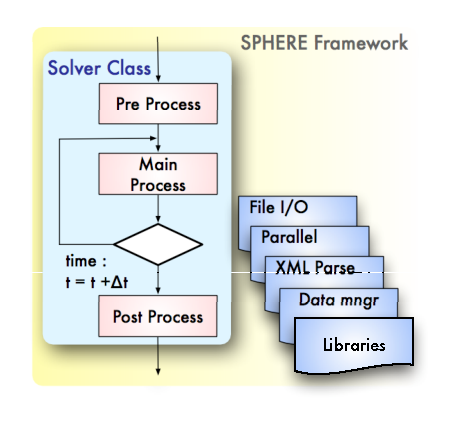
\includegraphics[width=8cm,clip]{Sphere_Control.eps}
\end{center}
\caption{V-Sphereの制御構造.プリ,メイン,ポストの処理プロセスが組み込まれており,提供されるライブラリ機能を用いてソルバークラスを構築します.}
\label{fig:Control structure}
\end{minipage} \hfill
\begin{minipage}{.47\textwidth}
\begin{center}
\includegraphics[width=7.5cm,clip]{DerivedClasses.eps}
\end{center}
\caption{差分プログラミングによるソルバークラスの開発.SklSolverBaseクラスから派生したFlowBaseクラスに共通機能をまとめ,このFBクラスを用いて目的のCBCソルバークラスを作成します.}
\label{fig:DerivedSolvers}
\end{minipage}
\end{figure}


V-Sphereの機能を用いて作成したアプリケーションはソルバークラスとしてV-Sphere自身に登録することができ,登録されたソルバークラス群は共通のユーザインターフェイスを備えたアプリケーションとして振る舞います.
\textbf{図\ref{fig:DerivedSolvers}}に示すようにSklクラス,SklBase\index{SklBase}クラス,およびSklSolverBaseクラスを提供します.
ここでは,SklSolverBaseクラスから流体解析に広く用いられる基本機能を抽出したFlowBaseクラスを作成しています.
ソルバークラスとしては,CBCクラスが派生し,さらにCBCクラスを継承してCPCソルバクラスが派生しています.
また,別の系統としてBCMソルバークラスが作成されています.
これらのソルバークラスは,例えば,シミュレートする物理現象や形状近似度,変数配置などが異なるソルバーですが,FlowBaseクラスにより統一的な振る舞いをします.
つまり,異なるソルバーであっても,ユーザーインターフェイスが統一されたアプリケーションとして構築することができます.

%
\section{CBCソルバークラス}
CBC(Cartesian based, Binary shape representation, Collocated)ソルバークラスは,V-Sphereコンポーネント群とクラスライブラリを利用して実装した非定常非圧縮性流体のソルバークラスです.
ソルバーを構築する上で必要な,パラメータハンドリング,主要な境界条件処理とパラメータの関連づけ,ファイル入出力,並列計算処理,組み込み例題など,コアアルゴリズム以外の部分は,FlowBaseクラスなどにパッケージ化しています.

CBCソルバークラスは,下記のような特徴を持っています.

\begin{description}
\item[ ] 形状近似   :キューブ近似(Binary Voxel)
\item[ ] 変数配置   :コロケート
\item[ ] 離散化    :有限体積法
\item[ ] 時間積分   :一次精度Euler陽解法%,二次精度Adams-Bashforth法,二次精度Crank-Nicolson法
\item[ ] 空間スキーム :一次精度風上,三次精度MUSCL%,二次精度中心,
\item[ ] 解法     :Fractional Step法
\item[ ] 反復法    :Jacobi緩和法, Point SOR, 2-colored SOR-SMA(ストライドメモリアクセス版)
%\item[ ]         2-colored SOR-CMA(連続メモリアクセス版)
\item[ ] スタート機能 :Initial(Impulsive, Smooth), 指定時刻からの再スタート
\item[ ] 入力ファイル :モデルファイル(svx, sbxフォーマット),XMLファイル(計算条件など)
\item[ ] 出力ファイル :sphフォーマット,履歴ファイル,モニター出力
\item[ ] 外部境界条件 :固定・移動壁面,流入,流出,周期,対称,トラクションフリー
\item[ ] 内部境界条件 :壁面,速度規定,流出,部分周期境界,圧力損失,多孔質
\item[ ] 温度境界条件 :断熱,熱伝導,熱伝達,輻射,熱流束,等温
\item[ ] 並列ライブラリ:mpich, mpich2, OpenMPI
\item[ ] 並列化    :等分割,多重連結領域分割
\item[ ] 組込み例題機能:キャビティフロー問題など,基本的な問題
\end{description}

